\documentclass[a4paper]{article}
\usepackage[margin=1.4in]{geometry}
\usepackage[T1]{fontenc}
\usepackage[utf8]{inputenc}
\usepackage{amsmath}
\usepackage{amssymb}
\usepackage{lmodern}
\usepackage[english]{babel}
\usepackage{graphicx}

\usepackage{tikz}
\usepackage{pgf-umlsd}
\usepackage{pgfplots}

\usetikzlibrary{arrows}
\usetikzlibrary{shapes.geometric, shadows}
\usetikzlibrary{patterns}
\usetikzlibrary{positioning}
\usetikzlibrary{external}
\usetikzlibrary{decorations.text}
\usetikzlibrary{plotmarks}
\pgfplotsset{compat=newest}

\usepgfplotslibrary{dateplot}

\renewcommand{\vec}[1]{\mathbf{#1}}

\begin{document}
	\begin{center}
		{\huge Bayesian estimates for trajectory matching} \\[2ex]
		{\large D\'aniel Kondor, Senseable City Lab, MIT} \\[1ex]
		{\large \today}
	\end{center}
	
	In this report I summarize some basic findings about estimating the probability of two spatial trajectories from two different datasets belonging
	to the same person. These complement the analysis in the upcoming manuscript~\cite{matchingpaper}. The main application is for the same two
	datasets described there. I use estimates based on the Bayes theorem:
	\begin{equation}
		P(A|B) = \frac{P(A)}{P(B)} P(B|A)
	\end{equation}
	The basic ideas are the same as in~\cite{Juhasz}, while the applicability of assumptions about independence among different events will not be
	applicable in our case.
	
	\section{Basic estimate}
	
		In our case we would like to estimate $P( \vec{x}_i \textrm{matches} \vec{y}_j | \textrm{data} )$, i.e.~the probability that trajectory
		$\vec{x}_i$ from dataset $X$ belongs to the same real person as trajectory $\vec{y}_j$ from dataset $Y$, given all the records we have in the
		two datasets, which is at this point represented by the abstract ``data'' requirement in the conditional. We apply Bayes theorem to this
		probability, gaining the following form:
		\begin{equation}
			P( \vec{x}_i \textrm{ matches } \vec{y}_j | \textrm{data} ) = \frac{ P( \vec{x}_i \textrm{ matches } \vec{y}_j ) }{ P( \textrm{data} ) }
				P( \textrm{data} | \vec{x}_i \textrm{ matches } \vec{y}_j )
		\end{equation}
		Here, we can estimate the three terms on the right hand side more easily. We can perform an estimation of $P( \textrm{data} | \vec{x}_i %
		\textrm{matches} \vec{y}_j )$ based on the datasets. The term $P( \vec{x}_i \textrm{ matches } \vec{y}_j )$ we identify as \emph{a priori}
		probabilities, i.e.~the probability that any two trajectories match in the two datasets without any further knowledge. We can simply define
		it to be $P( \vec{x}_i \textrm{ matches } \vec{y}_j ) = 1/N$, where $N$ is the number of individuals in either dataset $X$ or $Y$ or more
		generally, the population present in the area where the trajectories were recorded (this allows the datasets to be incomplete, e.g.~when
		they come from a service provider with a < 100\% market share in the area). The denominator, $P( \textrm{data} )$ denotes the probability of
		arriving at the datasets at hand; we can eliminate this by considering also the probability of $\vec{x}_i$ and $\vec{y}_j$ not being a match
		and exploiting that the two probabilities has to sum up to $1$ (i.e.~two trajectories either belong to the same person or not):
		\begin{equation}
			P( \vec{x}_i \textrm{ does not match } \vec{y}_j | \textrm{data} ) = \frac{ P( \vec{x}_i \textrm{ does not match } \vec{y}_j ) }{ P( \textrm{data} ) }
				P( \textrm{data} | \vec{x}_i \textrm{ does not match } \vec{y}_j )
		\end{equation}
		and
		\begin{equation}
			P( \vec{x}_i \textrm{ matches } \vec{y}_j | \textrm{data} ) + P( \vec{x}_i \textrm{ does not match } \vec{y}_j | \textrm{data} ) = 1
		\end{equation}
		Replacing both terms with the form obtained from the Bayes theorem, and using the shorthand notations for the conditional probabilities on the
		right hand sides: $P_T \equiv P( \textrm{data} | \vec{x}_i \textrm{ matches } \vec{y}_j )$ and $P_S \equiv P( \textrm{data} | \vec{x}_i %
		\textrm{ does not match } \vec{y}_j )$, we get the following expression:
		\begin{equation}
			P( \textrm{data} ) = \frac{P_T}{N} + \frac{N-1}{N}P_S
		\end{equation}
		where we also used the a priori probabilities $P( \vec{x}_i \textrm{ matches } \vec{y}_j ) = 1/N$ and $P( \vec{x}_i \textrm{ does not match } %
		\vec{y}_j ) = (N-1)/N$. This results in the following form for the original probability of match to be estimated:
		\begin{equation}
			P( \vec{x}_i \textrm{ matches } \vec{y}_j | \textrm{data} ) = \frac{P_T}{N} \frac{1}{ \frac{P_T}{N} + \frac{N-1}{N}P_S } =
				\frac{1}{1 + (N-1)\frac{P_S}{P_T}} = \frac{P_T}{P_T + (N-1)P_S}
			\label{mainestimate}
		\end{equation}
		In the following, the main challenge is estimating $P_T$ and $P_S$ realistically from the datasets.
	
	\section{Empirical match distributions}
		
		In this section, I base the estimation of $P_T$ and $P_S$ on the empirical distribution of getting a certain $m$ number of matches between a
		pair of users as estimated from the datasets (described in~\cite{matchingpaper}). The main approximation I use is that the difference between
		$P_T$ and $P_S$ is only whether the two trajectories ($\vec{x}_i$ and $\vec{y}_j$) actually belong to the same person or not. Note that $P_T$
		and $P_S$ actually includes the probability of getting all the records in both the datasets. In the following, I use $m$ to denote the number
		of matching records between the two trajectories (the criterion for matching is that the point are sufficiently close in both time and space).
		Note that $m$ is determined from the data, i.e.~it is a parameter for estimating the probabilities, being a part of the ``data'' abstraction.
		I assume that the trajectories have no inconsistent records (i.e.~points which are close in time but separated in space); if there are, then
		the probability of them being a true match can be trivially determined to be zero. In this section, I then proceed with writing these
		probabilities in product forms:
		\begin{gather}
			P_T = P_{ij}( m | \textrm{match} ) P ( \textrm{data} \setminus (\vec{x}_i, \vec{y}_j) | \textrm{match} ) \\
			P_S = P_{ij}( m | \textrm{not match} ) P ( \textrm{data} \setminus (\vec{x}_i, \vec{y}_j) | \textrm{not match} )
		\end{gather}
		In these cases, $P_{ij}$ is the probability of finding $m$ (spatially consistent) matches between the two trajectories ($\vec{x}_i$ and
		$\vec{y}_j$), given that these belong to the same person (``match'') or not (``not match''). The second terms in the products are the
		probabilities of getting the rest of the records in these cases. To be able estimate these, I make the following asusmptions:
		\begin{enumerate}
			\item $P ( \textrm{data} \setminus (\vec{x}_i, \vec{y}_j) | \textrm{match} ) = P ( \textrm{data} \setminus (\vec{x}_i, \vec{y}_j) | %
				\textrm{not match} )$, i.e.~the distribution describing the rest of the data does not depend on whether the two trajectories are a real
				match or not. This allows us to completely disregard this term, as it can be eliminated from equation~\ref{mainestimate}. Note that
				this is only an approximation; if the two trajectories are not a real match, both can have their true match in the other dataset,
				resulting in the trajectories having a higher number of matches with some other trajectory.
			\item The $P_{ij}$ distributions do not depend on the specific pair of trajectories selected, but only on the number of records in each of
				them. This is essentially the same assumption as the ones presented in Section~5.1. in the main manuscript~\cite{matchingpaper}. This
				assumption is necessary to estimate the probabilities from the empirical distributions in the data.
			\item The $P_{ij} (m | \textrm{match} )$ distribution essentially gives the probability of having $m$ \emph{temporal} matches between the
				matching trajectories of a person (since in this case it is assumed that all records are spatially consistent then). I then assume that
				this can be estimated with the empirical distribution of having $m$ temporal matches between the records of \emph{any} pair of
				trajectories from the two datasets, even if those are not spatially consistent.
		\end{enumerate}
		Based on these asusmptions, and omitting the second terms (which cancel out), the probabilities can be written in the following form, using the
		notations from Section~5.1. in~\cite{matchingpaper}:
		\begin{gather}
			P_T = P_t(m|r_i,r_j) \\
			P_S = P_s(m|r_i,r_j)
		\end{gather}
		Here, $P_t$ and $P_s$ are empirical distributions between groups of trajectories with $r_i$ and $r_j$ records as estimated from the data:
		$P_t(m|r_i,r_j)$ is the distribution of temporal matches between this group of trajectories, while $P_s(m|r_i,r_j)$ is the distribution of
		spatially consistent matches in this group. Using these estimates, I display the obtained probabilities for different user groups and number
		of matches in Fig.~\ref{bayes_est1}. We see that the probabilities display a rapid transition around 10-15 matching records (which correspong
		to about 50\% probability), while to reach high confidence, a significantly high number of matching records are required, i.e.~around or above
		30. Looking at Eq.~\ref{mainestimate}, we see that the main requirement of having a match with high confidence is that $P_T \gtrsim N P_S$,
		i.e.~the probability of the real match of the two trajectories has to be larger than the probability of a false positive match with \emph{any}
		of the $N$ trajectories in the dataset (note that an exact formula for having at least one false positive matching trajectory with any out of
		$N$ would be $1 - (1-P_S)^N \approx N P_S$ for $N P_S \ll 1$).
		
		\begin{figure}
			\centering
			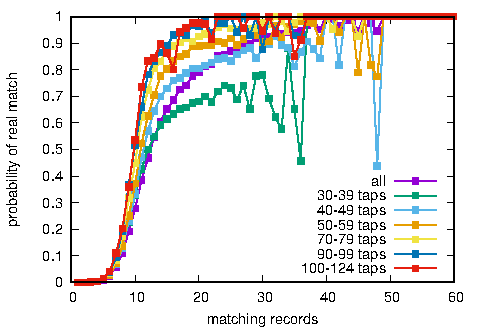
\includegraphics{bayes_est1}
			\caption{{\bf Average estimate probability of a true match between two trajectories as a function of the number of matching records.}
				Results are displayed as an average for all user records in the CDR dataset, while the separate lines show results for different
				groups of transportation users (the purple line is an average for any pair of trajectories in the two datasets).}
			\label{bayes_est1}
		\end{figure}
	
	
	\section{Independent individual points}	
		
		The main drawback of the previous approach is that it requires a good approximation of the $P_T$ and $P_S$ distributions based on empirical
		data. Especially for $P_S$ and a large number of matches, this becomes difficult as there are only a few such matching trajectories in the
		real dataset. This estimation seems much more problematic than estimating the $p_x$ average expected success ratios as done in Ref.~%
		\cite{matchingpaper}. Also, the estimation relies on average probabilities and thus cannot take into account individual differences in
		trajectories, e.g.~the fact that a matching pair of records in a less crowded area could be given more weight. For these reasons, it would be
		beneficial to have an estimate where probabilities are assigned to each record separately and combined together. In this section, I present
		the simplest such possible scenario, essentially the adaptation of the formulas in Ref.~\cite{Juhasz}, and then argue that the results are
		probably not correct as matching probabilities for separate records are not independent (i.e.~since people do not move uniformly randomly, but
		follow a given base routine).
		
		In the following, I use the shorthand notation $\vec{x}_i \sim \vec{y}_j$ to denote that the two trajectories belong to the same person and
		$\vec{x}_i \nsim \vec{y}_j$ to denote that they do not. Furthermore, I assume that the $\vec{x}_i$ trajectory has $r_i$ points, and denote
		by $z_k$ the total set of matching points around point $x_{ik}$ in trajectory $\vec{x}_i$ ($k \in 1,2,\ldots r_i$). In this scenario, I then
		assume that the $P_T$ and $P_S$ probabilities can be written as the products of individual probabilities corresponding to each point in the
		trajectories and then apply the Bayes theorem to each of these separately, essentially using the same approach as described in the Appendix
		of Ref.~\cite{Juhasz}:
		\begin{gather}
			P_T = \prod_{k=1}^{r_i} P ( z_k | \vec{x}_i \sim \vec{y}_j ) = \prod_{k=1}^{r_i} \frac{P(z_k)}{P( \vec{x}_i \sim \vec{y}_j)}
				P( \vec{x}_i \sim \vec{y}_j | z_k ) \\
			P_S = \prod_{k=1}^{r_i} P ( z_k | \vec{x}_i \nsim \vec{y}_j ) = \prod_{k=1}^{r_i} \frac{P(z_k)}{P( \vec{x}_i \nsim \vec{y}_j)}
				P( \vec{x}_i \nsim \vec{y}_j | z_k ) \\
			P( \vec{x}_i \sim \vec{y}_j | \textrm{data} ) = \frac{P( \vec{x}_i \sim \vec{y}_j )}{P( \textrm{data} )} P_T = 
				\frac{\prod P(z_k)}{P( \textrm{data} )} \frac{ \prod P( \vec{x}_i \sim \vec{y}_j | z_k ) }{ P( \vec{x}_i \sim \vec{y}_j)^{r_i-1}} \\
			P( \vec{x}_i \nsim \vec{y}_j | \textrm{data} ) = \frac{P( \vec{x}_i \nsim \vec{y}_j )}{P( \textrm{data} )} P_S = 
				\frac{\prod P(z_k)}{P( \textrm{data} )} \frac{ \prod P( \vec{x}_i \nsim \vec{y}_j | z_k ) }{ P( \vec{x}_i \nsim \vec{y}_j)^{r_i-1}}
		\end{gather}
		Again, the first factor can be eliminated using the relation that $P( \vec{x}_i \sim \vec{y}_j | \textrm{data} ) + P( \vec{x}_i %
		\nsim \vec{y}_j | \textrm{data} ) = 1$:
		\begin{equation}
			\frac{P( \textrm{data} )}{\prod P(z_k)} = \frac{ \prod P( \vec{x}_i \sim \vec{y}_j | z_k ) }{ P( \vec{x}_i \sim \vec{y}_j)^{r_i-1}} +
				\frac{ \prod P( \vec{x}_i \nsim \vec{y}_j | z_k ) }{ P( \vec{x}_i \nsim \vec{y}_j)^{r_i-1}}
		\end{equation}
		Using this, and performing some simplifications, and also using that $P( \vec{x}_i \sim \vec{y}_j | z_k ) + P( \vec{x}_i \nsim \vec{y}_j | z_k ) %
		= 1$ and $P( \vec{x}_i \sim \vec{y}_j) + P( \vec{x}_i \nsim \vec{y}_j) = 1$, we have the following result:
		\begin{equation}
			P( \vec{x}_i \sim \vec{y}_j | \textrm{data} ) =  \left ( 1 + \left ( \frac{P( \vec{x}_i \sim \vec{y}_j)}{1-P( \vec{x}_i \sim \vec{y}_j)}
				\right )^{r_i-1} \, \, \prod_{k=1}^{r_i} \frac{ 1 - P( \vec{x}_i \sim \vec{y}_j | z_k ) }{ P( \vec{x}_i \sim \vec{y}_j | z_k ) } \right )^{-1}
		\end{equation}
		Similarly to the previous case, we set $P( \vec{x}_i \sim \vec{y}_j) = 1 / N$, while the probability of having a match can be estimated very
		similarly to the scheme in Ref.~\cite{Juhasz}:
		\begin{equation}
			P( \vec{x}_i \sim \vec{y}_j | z_k ) = \begin{cases}
				\frac{1}{N} & \textrm{if no matching point for in } \vec{y}_j \textrm{ for } x_{ik} \\
				\frac{1}{p_k N} & \textrm{if } \exists y_{jl} \textrm{ spatially consistent match } x_{ik} - y_{jl} \\
				0 & \textrm{if } \exists y_{jl} \textrm{ impossible match } x_{ik} - y_{jl}
			\end{cases}
			\label{pointestimate}
		\end{equation}
		where $p_k$ is the ratio of spatially consistent matches to all temporal matches near point $x_{ik}$. The rationale for this choice is
		illustrated in Fig.~\ref{trsets} and is very similar to the way probabilities were estimated in Ref.~\cite{Juhasz} (see Fig.~4 there). For
		this discussion, we use the same definitions of matching as in the main manuscript (Ref.~\cite{matchingpaper}, see Section~4.1.): we define
		two records (from the two different datasets) to be a \emph{temporal match} if they are close to each other in time (closer than a threshold
		$\tau$, defined as five minutes when traveling by transit and ten minutes when walking). Among temporal matches, we refer to records as
		\emph{spatial matches} if their distance is less than a given $d$ threshold (chosen as 500 m for walking and 2 km for using transit). We refer
		to records outside this threshold a \emph{impossible matches}. In Eq.~\ref{pointestimate}, we are calculating the probability of trajectories
		$\vec{x}_i$ and $\vec{y}_j$ belonging to a same person, given only the knowledge about $z_k$, i.e.~the points in the neighborhood of
		$x_{ik} \in \vec{x}_i$. If trajectory $\vec{y}_j$ has no points as a temporal match there, then we learn no extra knowledge, resulting in
		using the a priory probability of $1/N$. In the case there is a point in the set of impossible matches, we can rule out them belonging to the
		same person, hence the probability becomes zero (and note that this will imply $P( \vec{x}_i \sim \vec{y}_j | \textrm{data} ) = 0$ as well).
		On the other hand, if the two trajectories have a spatial match, this provides further evidence for these to belong to the same person. The
		factor of $p_k$ then essentially represents a ``redistribution'' of probabilities: assuming that the total number of trajectories (in $Y$) is
		$N$, and we have $N^T_k$ with temporal matches, $N^I_k$ of these impossible, and $N^S_k$ spatial matches ($N^I_k + N^S_k = N^T_k$), then the
		total probability among $N^T_k$ trajectories is redistributed among only $N^S_k$, resulting in the $p_k \equiv N^S_k / N^T_k$ factor in
		comparison to the a priory probabilities.
		
		Using the probabilities from Eq.~\ref{pointestimate}, and noticing that we can eliminate the records from $\vec{x}_i$ which have no temporal
		matches in $\vec{y}_j$, we arrive at the following formula:
		\begin{equation}
			P( \vec{x}_i \sim \vec{y}_j | \textrm{data} ) = \frac{1}{1 + \left( \frac{1}{N-1} \right)^{m-1} \prod_{k=1}^m (p_k N - 1)}
		\end{equation}
		where trajectories $\vec{x}_i$ and $\vec{y}_j$ have $m$ spatially consistent matches, and $k = 1,2,\ldots m$ now indexes the $m$ records in
		$\vec{x}_i$ which have these matching points in $\vec{y}_j$. What remains in this case is that for each match, we have to characterize the
		neighborhood of each matching point. In the following, I show a simplified approximation where I assume that all $p_m$ ratios can be
		approximated from above. Clearly, if we assume that $p_m < p \forall m$, we have the following result for the estimate of the previous equation:
		\begin{equation}
			P( \vec{x}_i \sim \vec{y}_j | \textrm{data} ) > \frac{1}{1 + (N-1) \left (\frac{pN - 1}{N-1}\right)^m} \approx
				\frac{1}{1 + N p^m}
			\label{pointestimate2}
		\end{equation}
		where the last approximation is simply based on that $N \gg 1$ and $p \gg > 1/N$. Note that for a given $m$, the probability estimate will
		be increasing as $p$ decreases. In Fig.~\ref{bayes_est2}, I display the result in Eq.~\ref{pointestimate2} along with the previous estimate as
		well. We see that estimates calculated from Eq.~\ref{pointestimate2} give much higher values for match probabilities than the previous approach
		which based estimates on the empirical distribution of matches among trajectories in the data. I believe that the previouy methodology is more
		correct and the results based on Eq.~\ref{pointestimate2} actually overestimate the real probabilities. The main approximation which is
		questionable is writing $P_T$ and $P_S$ as a product of independent probabilities for each record in $\vec{x}_j$. While in the case of $P_T$,
		this could be justified by the assumptions that generating a record in the two datasets is independent, but in the case of $P_S$, the
		probability of record pairs being spatially consistent is not independent: we can argue that this depends on a latent parameter whether the
		people generating the two trajectories have similar mobility habits (i.e.~live and work relatively close to each other), as human mobility in
		general shows high regularity.
		

\def \firstcircle  {(0,0) circle (3cm)}
\def \secondcircle {(0,0) circle (2cm)}
\def \thirdcircle  {(0,0) circle (1cm)}
\begin {figure}
\centering
\resizebox {0.45\textwidth} {!} {\begin {tikzpicture}
    \draw (-3.8,-3.8) rectangle (3.8,3.8) node [pos=.9, xshift=-1cm, yshift=.4cm] {};
    \draw [fill = black!20!white] \firstcircle node[above = 2.2cm] {};
    \draw [fill = white, cm = {cos(-90), -sin(-90), sin(-90), cos(-90), (0,0)}, postaction = {decorate}, decoration = {raise = -3.6ex, text along path, text align = center, text = {All trajectories in Y}}] \secondcircle node [above = 1.2cm] {};
    \draw [fill = black!70!white,
cm = {cos(-90), -sin(-90), sin(-90), cos(-90), (0,0)}, postaction = {decorate}, decoration = {raise = -3.6ex, text along path, text align = center, text = {Inconsistent temporal matches}}] \thirdcircle node [align = center,  font = \small, text = white] {Spatially\\consistent\\matches}; \end {tikzpicture}}
\caption {{\bf Relation of the different types of trajectories.} The sets correspond to trajectories from $Y$ with relation to one point $x_{ik}$ from
	a trajectory in $X$. The darker the subset is, the higher the probability of a match. See Fig.~4 and the related discussion in Ref.~\cite{Juhasz}
	for reference.}
	\label {trsets}
\end {figure}

		\begin{figure}
			\centering
			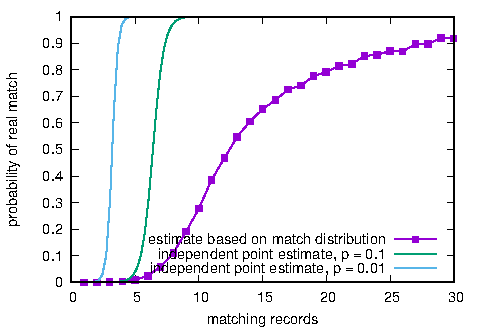
\includegraphics{bayes_est2}
			\caption{{\bf Average estimate probability of a ture match between two trajectories as a function of the number of matching records.}
				The two lines are based on Eq.~\ref{pointestimate2}, with $p$ values of $0.1$ and $0.01$ (the smaller value results in higher
				probabilities. We expect real $p_m$ values to be even smaller, but these values already result in much higher match probabilities
				than the previous estimation method. The previous estimate (the same data as in Fig.~\ref{bayes_est1}) is shown for comparison.}
			\label{bayes_est2}
		\end{figure}
		

\begin{thebibliography}{9}
	\bibitem{matchingpaper}	Kondor D, Hashemian B, de Montjoye YA, Ratti C (2017).
		Towards matching user mobility traces in large-scale datasets. \emph{manuscript in preparation}
		\texttt{https://www.dropbox.com/s/gm51conqrvalv4z/bigdatapaper\_merged.pdf?dl=0}
	\bibitem{Juhasz} Juhász PL, Stéger J, Kondor D, Vattay G (2016).
		A Bayesian Approach to Identify Bitcoin Users.
		\texttt{arXiv:1612.06747}. Retrieved from \texttt{http://arxiv.org/abs/1612.06747}
\end{thebibliography}

		
\end{document}
